\subsection{归并排序mergesort}
\subsubsection{算法类别}
mergesort(归并排序)是一种基于\textbf{分治}的算法.

\subsubsection{算法思路}
在mergesort中, 待排序数组被分为两等分, 分别排序后合并为一个数组. \par
mergesort是一个递归算法, 持续的将数组二等分并对等分后得到的两个数组
分别进行mergesort, 直到数组不能再分, 此时数组为空或仅剩1个元素.
也就是说, 这是递归的终止情况. 如果数组有多个元素, 将数组分为两等份,
并在每一份上递归的调用mergesort. 最终, 当两半数组都被排序, 对两个数组
执行merge(合并)操作. \par
merge(合并)操作是将两个较小的有序数组结合成一个大的有序数组的过程.

\subsubsection{关键函数及代码段的描述}
采用non-recursive的迭代方式实现mergesort, 基于DRY \footnote{
	DRY: don't repeat yourself, 即不要做重复性的工作,
	通过良好的函数和类的抽象减少冗余和重复代码的出现}
的原则, 将mergesort分为三个函数, 分别是mergeSort(), mergePass(int *x,
int *y, int s, int n)和merge(int *c, int *d, int l, int m, int r). \par
mergeSort()是归并排序的入口函数, 管理步长倍增, 并通过将数组a和数组
b交替作为辅助数组的方式, 减少了一半的元素赋值操作. \par
mergePass()是归并排序中的一遍, 通过不断调用merge(),
将两个子序列用步长s按从小到大的顺序排序. \par
merge()函数将两个子数组c[l, ..., m]和c[m+1, ..., r]合并到d中. \par
函数均使用类似C++的Pseudo-Code描述.
\begin{lstlisting}[language=c++]
/**
 * Iterative mergesort function to sort a[0, ..., n-1], 
 * Merge subarrays in bottam up manner. First merge subarrays of
 * size 1 to create sorted subarrays of size 2, then merge subarrays
 * of size 2 to create sorted subarrays of size 4, and vice versa.
 */
void mergeSort() {
	// Initializing...
	int s = 1;
	while (s < n) {
		// treat b as assistant array
		mergePass(a, b, s, n);
		// double the step size
		s += s;
		// treat a as assistant array
		mergePass(b, a, s, n);
		// double the step size
		s += s;
	}
}

/**
 * A pass of merge with step size of s.
 */
void mergePass(int *x, int *y, int s, int n) {
	int i = 0; // left variable
	// merge until less than 2*s elements left.
	if (i + step_size - 1 < n) {
		merge till the end of array
	} else {
		append rest elements of x to y
	}
}

/**
 * Function to merge the two halves c[l, ..., m] and c[m+1, ..., r]
 * to d
 */
void merge(int *c, int *d, int l, int m, int r) {
	int i = l;
	int j = m+1;
	int k = i;
	// merge the two halves of array c to array d
	while(left half not reach the end &&
		right half of c not reach the end) {
			 append smaller element of c[i] and c[j] to d[k]
			 and increase i and k or j and k
		}

	// if left half of array c reaches the end, append rest elements
	// of right half of array c to d
	if (i > m) {
		append rest elements of right half of array c to d
	} else {
		vice versa
	}
}
\end{lstlisting}

\subsubsection{算法时间及空间复杂性分析}
\paragraph{空间复杂度分析}
mergesort需要一个长度为n的辅助数组进行辅助merge, 故空间复杂度为$O(n)$.

\paragraph{时间复杂度分析}
对于mergesort, 比较和挪动元素都发生在merge阶段, 由于对两个元素不进行
比较就不可能进行挪动, 故元素移动次数不会大于比较次数, 只需根据比较次数
即可分析时间复杂度. \par
由于归并排序是递归的过程, 可以方便地写出递推式:
\begin{align}
	C(1)       & = 0                                \nonumber \\
	C_{max}(n) & = 2C(\frac{n}{2}) + n-1            \nonumber \\
	C_{min}(n) & = 2C(\frac{n}{2}) + \frac{n}{2}    \nonumber \\
	C_{avg}(n) & = 2C(\frac{n}{2}) + \frac{3n-2}{2} \nonumber
\end{align}
令\(n=2^k\), 将式中$O(n)$项
用$O(n)$代替, 则最好, 最坏和平均情形都为相同形式, 即
\begin{equation}
	C(n) = 2C(\frac{n}{n})+(n)
\end{equation}
记$C(n)$为比较次数, 有
\begin{gather}
	C'(0) = 0            \nonumber \\
	C'(k) = 2C'(k-1)+2^k \nonumber
\end{gather}
得
\begin{equation}
	C'(k) = 2^kC'(0)+k\cdot 2^k = k\cdot 2^k \nonumber
\end{equation}
即
\begin{equation}
	C(n) = n\log_2{n} \nonumber
\end{equation}
综上, mergesort的时间复杂度为$O(n\log{n})$

\subsection{应用尾递归优化的快速排序quicksort}
\subsubsection{算法类别}
quicksort(快速排序)和mergesort一样, 也是一种\textbf{分治法}算法.

\subsubsection{算法思路}
\label{sec:quicksortThink}
\paragraph{概述}
quicksort将一个元素作为\textbf{pivot(枢轴)}, 并将给定数组围绕着pivot
进行划分. 对pivot的选取方式有很多种:
\begin{itemize}
	\item 总是选取第一个元素作为pivot.
	\item 总是选取最后一个元素作为pivot.
	\item 随机选取一个元素作为pivot.
	\item 选取中间元素作为pivot.
\end{itemize}
选取合适的pivot, 有利于提高quicksort的健壮性, 减少退化\footnote{退化:
	指quicksort退化到$O(n)$时间复杂度的情形, 这会出现在每次partition都只能分
	出常数个而不是一定比例个元素的情形.}现象的发生.\par
quicksort的关键阶段是partition(). partitions的目标是, 给定一个数组和其中
的一个元素x作为pivot, 将x放在排好序数组里它应该在的位置, 将所有小于x的
元素放在x前面, 所有不小于x的元素放在x的后面. 这所有的过程都应该在线性时间
内完成. \par
此外, 由于quicksort是\textbf{尾递归}的, 所以可以方便的进行尾递归优化\footnote{
	尾递归优化: 将尾递归调用函数展开为while循环, 从而减少递归调用的次数}, 从而将最坏
情况空间复杂度降到$O(\log{n})$.
\begin{figure}[h!]
	\centering
	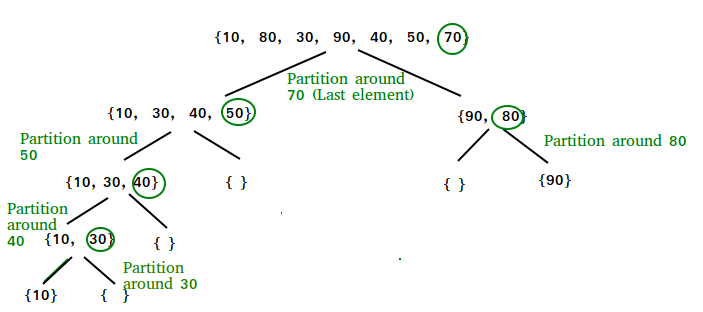
\includegraphics[width=0.8\textwidth]{figures/QuickSort2.png}
	\caption{Quicksort中的partition过程}
\end{figure}
\paragraph{Partition算法}
在quicksort中有许多种partition算法, 我采用的是一种从最左边元素开始, 跟踪
较小元素的下标i. 在循环的过程中, 如果找到一个小于x的元素,
将目前的元素和arr[i]进行交换; 否则, 不进行操作的方法.

\subsubsection{关键函数及代码段的描述}
递归的quickSort()函数作为quicksort调用的入口, 使用尾递归调用优化来确保最坏
情况下$O(\log{n})$的空间复杂度.\par
partition()函数是quicksort的核心部分, 将数组元素围绕pivot按大小进行划分.\par
对函数均使用类似C++的Pseudo-Code描述.
\begin{lstlisting}[language=c++]
/**
 * Main function to perform quicksort on arr[],
 * optimized with **tail call elimination**
 */
void QuickSort::quickSort(int arr[], int l, int h) {
    while (l < h) {
        // Median of arr[]
        int pivor = arr[(l + h) / 2];

        // Partition the array around median
        int p = partition(arr, l, h, pivor);

        // If left half has less elements, recur for left half.
        // Else recur for right half.
        if (p - l < h - p) {
            quickSort(arr, l, p - 1);
            l = p + 1;
        } else {
            quickSort(arr, p + 1, h);
            h = p - 1;
        }
    }
}

// Search for x in arr[l, ..., r], then partition
// arr[] around x.
int QuickSort::partition(int arr[], int l, int r, int x) {
    int i = 0;
    // Search for x in arr[l, ..., r], if found, move it to end
    for (i = l; i < r; i++) {
        if (arr[i] == x) {
            break;
        }
    }
    swap arr[i] and arr[r];

    // Make partition
    i = l;
    for (int j = l; j <= r - 1; j++) {
        if (arr[j] <= x) {
            swap arr[i] and arr[j];
            i++;
        }
    }
    swap arr[i] and arr[r]
    return i;
}
\end{lstlisting}

\subsubsection{算法时间及空间复杂性分析}
\paragraph{空间复杂度分析}
\label{par:quicksortSpace}
由于quicksort主要操作都在分区partition()函数中, 而partition()函数
是原地(in-place)的, 故quicksort是原地排序算法(in-place algorithm),
不占用额外空间, 空间复杂度为O(1).\par
\textbf{然而}, 递归实现的quicksort函数会递归的两次调用自身, 在最坏
情况下会占用$O(n)$的函数调用栈上空间(与下面的时间复杂度最坏情况分析过程相同).\par
为了解决这个问题, 我使用了\textbf{尾递归优化}的方式, 改写quicksort使其
只执行一次递归调用, 即上面代码中的quickSort(), 并且, 即便在最坏的,
数组被划分为左半部分总有$n-1$个元素的情况下, quickSort()总会对较小数组部分
进行递归调用, 而对较大数组部分进行迭代调用. 这样可以保证在所有递归调用中,
也只使用$O(log{n})$的额外空间.

\paragraph{时间复杂度分析}
\label{par:quicksortTime}
由于quicksort不进行比较就不会移动元素, 所以元素移动次数一定小于比较次数,
像mergesort的分析过程一样, 只需要分析比较次数即可.\par
由于快速排序是递归的过程, 可以方便地写出递推式:
\begin{align}
	C(1)       & = 0                        \nonumber \\
	C_{min}(n) & = 2C(\frac{n}{2}) + n - 1  \nonumber \\
	C_{max}(n) & = C(1) + C(n - 1) + n - 1  \nonumber
\end{align}
令\(n=2^k\), 将式中$O(n)$项用$O(n)$代替, 得
\begin{align}
	C'(0)       & = 0                                           \nonumber \\
	C'_{min}(k) & = 2C'_{avg}(k-1)+2^k-1                        \nonumber \\
	            & = 2C'_{avg}(0)+k\cdot 2^k - \sum_{i=0}^k 2^i  \nonumber \\
	            & = k\cdot 2^k - 2^{k+1}+1                      \nonumber \\
	            & = (k-2)\cdot 2^k + 1 \nonumber
\end{align}
故
\begin{align}
	C_{min}(n) & = (\log_2{n}-2)\cdot n+1  \nonumber \\
	C_{max}(n) & = \sum_{i=1}^{n-1}i       \nonumber \\
	           & = \frac{n(n-1)}{2}        \nonumber \\
	           & =\frac{n^2-n}{2}          \nonumber
\end{align}
综上, quicksort的平均时间复杂度为$O(n\log n)$, 最坏时间复杂度为
$O(n^2)$.

\subsection{应用线性时间选择优化的快速排序quicksort}
\subsubsection{算法类别}
quicksort(快速排序)和mergesort一样, 也是一种\textbf{分治法}算法.
k'th smallest element in unsorted array(线性时间选择)也是一种
\textbf{分治法}算法.

\subsubsection{算法思路}
线性选择优化并不改变quicksort的思路, 故本节主要介绍线性选择问题的思路.

\paragraph{quicksort部分}
参考上面的分析~\ref{sec:quicksortThink}.

\paragraph{线性时间选择问题}
如果能在线性时间内找到一个划分基准,使得按这个基准所划分出的2个子数组
的长度都至少为原数组长度的$\epsilon$ 倍($0<\epsilon <1$是某个正常数),那么就可以在最坏情况
下用O(n)时间完成选择任务,这是线性时间选择问题。\par
寻找第k小元素的函数kthSmallest(arr[0, ..., n-1], k)的大致流程如下.
\begin{enumerate}
	\item 将数组划分为含最多5个元素的小数组.
	\item 将前面创建的n/5个小数组分别排序, 找到每个小数组的中位数. 这一步
	      可以选用任意的排序算法, 例如Insertion sort(插入排序). 在这一步之后,
	      产生一个数组median[], 包含所有n/5个小数组的中位数.
	\item 找到kthSmallest(median[0, ..., n/5-1], n/10).
	\item 递归的找到median[]数组的kthSmallest.
\end{enumerate}

\subsubsection{关键函数及代码段的描述}
quickSort()是对arr[]进行quicksort的入口, 用kthSmallest算法寻找中位数作为
pivot, 从而避免了退化.\par
kthSmallest()递归地寻找arr[]中的k'th最小元素, 最坏情况下只使用线性时间.\par
findMedian()使用插入排序寻找数组的中位数. 在本算法中只对大小为5的数组使用.\par
partition()对数组arr[]根据pivot x进行分区.\par
函数均使用类似C++的Pseudo-Code进行描述.
\begin{lstlisting}[language=c++]
/**
 * Main function to perform quicksort on arr[],
 * optimized with **tail call elimination**
 */
void QuickSort::quickSort(int arr[], int l, int h) {
    while (l < h) {
        int n = size of current subarray;

        int med = find median of arr[] using kthSmallest();

        // Partition the array around median
        int p = partition(arr, l, h, med);

        // tail recursive call elimination
        if (p - l < h - p) {
            quickSort(arr, l, p - 1);
            l = p + 1;
        } else {
            quickSort(arr, p + 1, h);
            h = p - 1;
        }
    }
}

/**
 * recursively find kth smallest element in arr[]
 * in worst linear time
 */
int QuickSort::kthSmallest(int arr[], int l, int r, int k) {
    // Indeces range from 1.
    if (k is smaller than number of elements in array) {
        int n = number of elements in arr.

        int i = 0;
        Divide arr[] in groups of size 5, then store median
        of each group in median[] array with findMedian()

        // Recursively find median of all medians.
        int medOfMed =
            (i == 1) ? median[0] : kthSmallest(median, 0, i - 1, i / 2);

        int pos = partition(arr, l, r, medOfMed);

        if (pos - l == k - 1) {
            return arr[pos];
        } else if (pos - l > k - 1) {
            return kthSmallest(arr, l, pos - 1, k);
        }

        return kthSmallest(arr, pos + 1, r, k - (pos - l) - 1);
    }

    // If k is more than number of elements in arr[]
    return INT_MAX;
}

// A simple function to find median of arr[]. This is called
// only for an array of size 5 in this program, thus has an
// time complexity of O(1).
int QuickSort::findMedian(int arr[], int n) {
  	Simple insertion sort on arr[];

    return arr[n / 2];
}

// Search for x in arr[l, ..., r], then partition
// arr[] around x.
int QuickSort::partition(int arr[], int l, int r, int x) {
    int i = 0;
    Search for x in arr[l, ..., r];
    if (found) {
			swap arr[i] and arr[r];
    }

    // Make partition
    i = l;
    for (int j = l; j <= r - 1; j++) {
        if (arr[j] <= x) {
            swap arr[i] and arr[j];
            i++;
        }
    }
  	swap arr[i] and arr[r];
    return i;
}
\end{lstlisting}

\subsubsection{算法时间及空间复杂性分析}
\paragraph{空间复杂度分析}
由于与上面的quicksort采用了相同的尾递归调用优化, 同样有$O(log{n})$的
考虑函数调用栈上空间占用的空间复杂度, 参见~\ref{par:quicksortSpace}\par
对于线性选择问题部分, 使用了大小为$\lceil\frac{n}{5}\rceil$的辅助数组,
空间复杂度为$O(n)$.

\paragraph{时间复杂度分析}
对于\textbf{quicksort}部分的时间复杂度分析, 参见~\ref{par:quicksortTime}.\par

对于\textbf{线性选择问题}部分, 最坏情况下的时间复杂度为$O(n)$.\par
寻找长度为5的数组的中位数花费$O(1)$时间, 由于有$n/5$个长度为5的数组,
这一步花费$O(n)$时间.\par
寻找median[]数组的中位数花费了$T(n/5)$的时间. 之后进行的partition操作
花费$O(n)$时间.\par
对于kthSmallest()最后的递归调用部分, 最坏情况是最大元素数量比medOfMed大
或者比medOfMed小.\par
在median[]数组中, 至少有一半的元素应该不小于medOfMed.
因此, 至少$n/5$个组中的一半有3个比medOfMed大的元素, 不考虑有数组元素个数
小于5个的情况下. 因此, 比medOfMed大的元素数目至少为
\begin{equation}
	3([\frac{1}{2}\lceil\frac{n}{5}\rceil]-2)\geq\frac{3n}{10}-6
	\label{eq:kthSmallest1}
\end{equation}
类似的, 小于medOfMed的元素数量也至少是$\frac{3n}{10}-6$. 在最坏情况下,
函数递归调用最多$n-(\frac{3n}{10}-6)$次, 也就是$\frac{7n}{10}+6$个元素.\par
解$\frac{7n}{10}+6<20$得所有不大于80个元素的输入都可以在O(1)时间内找到
中位数. 因此, 有
\begin{equation}
	T(n) \leq
	\begin{cases}
		\Theta(1),                                          & \text{ if }n \leq 80 \\
		T(\lceil\frac{n}{5}\rceil)+T(\frac{7n}{10}+6)+O(n), & \text{ if }n > 90
	\end{cases}
	\label{eq:kthSmallest2}
\end{equation}
对常数$C$和任意的$n>80$, 有
\begin{align}
	T(n) & \leq c\frac{n}{5}+c(\frac{7n}{10}+6)+O(n)  \nonumber \\
	     & \leq c\frac{n}{5}+c+c\frac{7n}{10}+6c+O(n) \nonumber \\
	     & \leq c\frac{9n}{10}+7c+O(n)                \nonumber \\
	     & \leq cn \nonumber
	\label{eq:kthSmallest3}
\end{align}
综上, 这个算法是线性的.\par
\textbf{然而}, 由于这个算法中的常数c很大, 导致虽然最坏情况下时间复杂度更低,
但是实际应用中的表现却不好, 参见~\ref{sec:sortBench}.\par
